\documentclass[final,onefignum,onetabnum]{siamart220329}

%% ------------------------------------------------------------------
%% Code used in examples, needed to reproduce 
%% ------------------------------------------------------------------
%% Used for \set, used in an example below
\usepackage{braket,amsfonts}

%% Used in table example below
\usepackage{array}

%% Used in table and figure examples below
\usepackage[caption=false]{subfig}
%% Used for papers with subtables created with the subfig package
\captionsetup[subtable]{position=bottom}
\captionsetup[table]{position=bottom}

%% Used for PgfPlots example, shown in the "Figures" section below.
\usepackage{pgfplots}

%% Used for creating new theorem and remark environments
\newsiamthm{claim}{Claim}
\newsiamremark{remark}{Remark}
\newsiamremark{hypothesis}{Hypothesis}
\crefname{hypothesis}{Hypothesis}{Hypotheses}

%% Algorithm style, could alternatively use algpseudocode
\usepackage{algorithmic}

%% For figures
\usepackage{graphicx,epstopdf}

%% For referencing line numbers
\Crefname{ALC@unique}{Line}{Lines}

%% For creating math operators
\usepackage{amsopn}
\DeclareMathOperator{\Range}{Range}

% Custom
\usepackage[utf8]{inputenc}
\usepackage[english]{babel}
% Math packages
\usepackage{amsmath}
\usepackage{amsfonts}
\usepackage{amssymb}

\newcommand{\bn}{\bold{n}}
\newcommand{\bx}{\boldsymbol{x}}
\newcommand{\bhx}{{\bold{\hat{x}}}}
\newcommand{\bhy}{\bold{\hat{y}}}
\newcommand{\hx}{{\hat{x}}}
\newcommand{\hy}{{\hat{y}}}
\newcommand{\hvarphi}{{\hat{\varphi}}}
\newcommand{\hPhi}{{\hat{\Phi}}}
\newcommand{\by}{\boldsymbol{y}}
\newcommand{\br}{\boldsymbol{r}}
\newcommand{\btheta}{\bold{\theta}}
\newcommand{\htau}{{\hat{\tau}}}
\newcommand{\hpsi}{{\hat{\psi}}}
\newcommand{\M}{\mathcal{T}}
\newcommand{\tensor}[1]{\overline{\overline{\boldsymbol{#1}}}}
\newcommand{\chia}{\chi^{\text{affine}}}
\newcommand{\pt}{\bold{P}}
\newcommand{\uapprox}{u^{\text{approx}}}
\newcommand{\uref}{u^{\text{ref}}}

\newcommand{\bol}{\boldsymbol}
\newcommand{\nee}{\bold{e}}
\newcommand{\nej}{\bold{j}}
\newcommand{\nem}{\bold{m}}
\newcommand{\nephi}{\boldsymbol{\phi}}
\newcommand{\nepsi}{\boldsymbol{\psi}}
\newcommand{\new}{\boldsymbol w}
\newcommand{\ney}{\boldsymbol{y}}
\newcommand{\nex}{\boldsymbol{x}}
\newcommand{\bnex}{\bold{x}}
\newcommand{\nez}{\boldsymbol{z}}
\newcommand{\nev}{\boldsymbol{v}}
\newcommand{\neu}{\boldsymbol{u}}
\newcommand{\nerho}{\boldsymbol{\varrho}}
\newcommand{\ner}{\bol{r}}
\newcommand{\TE}{\mathrm{TE}}
\newcommand{\TM}{\mathrm{TM}}
\newcommand{\de}{\,\mathrm{d}}
\newcommand{\e}{\operatorname{e}}
\newcommand{\im}{\operatorname{i}}
\newcommand{\inc}{\mathrm{inc}}
\newcommand{\rad}{\mathrm{rad}}
\newcommand{\gui}{\mathrm{gui}}
\newcommand{\ontext}{\quad\mbox{on}\quad}
\newcommand{\intext}{\quad\mbox{in}\quad}
\newcommand{\andtext}{\quad\mbox{and}\quad}
\newcommand{\dtn}{\mathcal{B}}
\newcommand{\dtnn}{\mathrm{T}}
\newcommand{\sovo}{\operatorname{H}}
\newcommand{\keps}{k_{\varepsilon}}
\newcommand{\p}{\partial}
\newcommand{\cp}{\times}
\newcommand{\mpt}{\mathbf A}
\newcommand{\crt}{\mathbf J}
\newcommand{\dygfn}{\bar{\bold G}}
\newcommand{\untx}{\hat x}
\newcommand{\unty}{\hat y}
\newcommand{\untz}{\hat z}
\newcommand{\teps}{\boldsymbol{\overline\epsilon}}
\newcommand{\tmu}{\boldsymbol{\overline\mu}}
\newcommand{\ftr}{\widehat{F}}
\newcommand{\dlpfs}{\bold{K}^{\mathrm{fs}}}
\newcommand{\dlphs}{\bold{K}^{\mathrm{hs}}}
\newcommand{\slpfs}{\bold{S}^{\mathrm{fs}}}
\newcommand{\slphs}{\bold{S}^{\mathrm{hs}}}
\newcommand{\real}{\mathrm{Re}\,}
\newcommand{\uinc}{u_{\mathrm{inc}}}
\newcommand{\imag}{\mathrm{Im}\,}
\newcommand{\inte}{\mathrm{int}}
\newcommand{\exte}{\mathrm{ext}}
\newcommand{\lf}{\left}
\newcommand{\rg}{\right}
\newcommand{\tdir}{\widehat{\boldsymbol \theta}}
\newcommand{\rdir}{\widehat{\boldsymbol r}}
\newcommand{\xdir}{\widehat{\bold i}}
\newcommand{\ydir}{\widehat{\bold j}}
\newcommand{\zdir}{\widehat{\bold k}}
\newcommand{\R}{\mathbb{R}}
\newcommand{\C}{\mathbb{C}}
\newcommand{\N}{\mathbb{N}}
\newcommand{\elc}{\mathbf E}
\newcommand{\mgn}{\mathbf H}
\newcommand{\mgf}{\bold H}
\newcommand{\elf}{\bold E}
\newcommand{\can}{\bold e}
\newcommand{\normal}{n}
\newcommand{\nor}{\bold n}
\newcommand{\curl}{\operatorname{curl}}
\newcommand{\grd}{\operatorname{grad}}
\newcommand{\dv}{\operatorname{div}}
\newcommand{\vecphi}{\boldsymbol{\upphi}}

\newcommand{\Dcal}{\mathcal{D}}
\newcommand{\Gcal}{\mathcal{G}}
\newcommand{\Hcal}{\mathcal{H}}
\newcommand{\Ical}{\mathcal{I}}
\newcommand{\Lcal}{\mathcal{L}}
\newcommand{\Mcal}{\mathcal{M}}
\newcommand{\Ocal}{\mathcal{O}}
\newcommand{\Pcal}{\mathcal{P}}
\newcommand{\Qcal}{\mathcal{Q}}
\newcommand{\Scal}{\mathcal{S}}
\newcommand{\Wcal}{\mathcal{W}}
\newcommand{\Tcal}{\mathcal{T}}
\newcommand{\Kcal}{\mathcal{K}}
\newcommand{\tG}{\mathbb{G}}
\newcommand{\tId}{\mathbb{I}}
\newcommand{\Tbf}{\mathbf{T}}

\newcommand{\bigo}[1]{\Ocal\left(#1\right)}
\newcommand{\abs}[1]{\left|#1\right|}
\newcommand{\norm}[1]{\left\|#1\right\|}

%% ------------------------------------------------------------------
%% Macros for in-document examples. These are not meant to reused for
%% SIAM journal papers.
%% ------------------------------------------------------------------
\usepackage{xspace}
\usepackage{bold-extra}
\usepackage[most]{tcolorbox}
\newcommand{\BibTeX}{{\scshape Bib}\TeX\xspace}
\newcounter{example}
\colorlet{texcscolor}{blue!50!black}
\colorlet{texemcolor}{red!70!black}
\colorlet{texpreamble}{red!70!black}
\colorlet{codebackground}{black!25!white!25}

\newcommand\bs{\symbol{'134}} % print backslash in typewriter OT1/T1
\newcommand{\preamble}[2][\small]{\textcolor{texpreamble}{#1\texttt{#2 \emph{\% <- Preamble}}}}

\lstdefinestyle{siamlatex}{%
  style=tcblatex,
  texcsstyle=*\color{texcscolor},
  texcsstyle=[2]\color{texemcolor},
  keywordstyle=[2]\color{texemcolor},
  moretexcs={cref,Cref,maketitle,mathcal,text,headers,email,url},
}

\tcbset{%
  colframe=black!75!white!75,
  coltitle=white,
  colback=codebackground, % bottom/left side
  colbacklower=white, % top/right side
  fonttitle=\bfseries,
  arc=0pt,outer arc=0pt,
  top=1pt,bottom=1pt,left=1mm,right=1mm,middle=1mm,boxsep=1mm,
  leftrule=0.3mm,rightrule=0.3mm,toprule=0.3mm,bottomrule=0.3mm,
  listing options={style=siamlatex}
}

\newtcblisting[use counter=example]{example}[2][]{%
  title={Example~\thetcbcounter: #2},#1}

\newtcbinputlisting[use counter=example]{\examplefile}[3][]{%
  title={Example~\thetcbcounter: #2},listing file={#3},#1}

\DeclareTotalTCBox{\code}{ v O{} }
{ %fontupper=\ttfamily\color{texemcolor},
  fontupper=\ttfamily\color{black},
  nobeforeafter,
  tcbox raise base,
  colback=codebackground,colframe=white,
  top=0pt,bottom=0pt,left=0mm,right=0mm,
  leftrule=0pt,rightrule=0pt,toprule=0mm,bottomrule=0mm,
  boxsep=0.5mm,
  #2}{#1}

% Stretch the pages
\patchcmd\newpage{\vfil}{}{}{}
\flushbottom

%% ------------------------------------------------------------------
%% End of macros for in-document examples. 
%% ------------------------------------------------------------------

%% ------------------------------------------------------------------
%% HEADING INFORMATION
%% ------------------------------------------------------------------
\title{Just another implementation of the Fast Multipole Method for the electrostatic potential in 2D}

\author{Rodrigo Arrieta\thanks{Mathematics Department, Massachusetts Institute of Technology, Cambridge, MA 02139,
		United States (\email{rarrieta@mit.edu}).}}


%% ------------------------------------------------------------------
%% END HEADING INFORMATION
%% ------------------------------------------------------------------

%% ------------------------------------------------------------------
%% MAIN Document
%% ------------------------------------------------------------------
\begin{document}
\maketitle

%% ------------------------------------------------------------------
%% ABSTRACT
%% ------------------------------------------------------------------
\begin{abstract}
\end{abstract}

%% ------------------------------------------------------------------
%% END HEADER
%% ------------------------------------------------------------------

\section{Introduction}
\label{sec:intro}
%source \cite{martinsson2019fast}

\section{The multipole expansion for well separated clusters of points}\label{sec:multipole}

Consider the electrostatic potential $\{u_i\}_{i=1}^M \subset \R$ at some target points $\{\bol{x}\}_{i=1}^M \subset \R^2$ generated by a set of point charges $\{q_j\}_{j=1}^N \subset R$ located at source points $\{\bol y_j\}_{j=1}^N$. Mathematically, this is expressed as
\begin{align}
	u(\bol x_i) := u_i = \sum_{j=1}^{N} G(\bol x_i, \bol y_j)q_j, \quad i = 1,2,\dots,M, \label{eq:dir_pot}
\end{align}
where the kernel $G$ is taken as a scaled version of the fundamental solution of the Laplace equation in two dimensions,
\begin{align}
	G(\bol x, \bol y) = \begin{cases}
		\log \abs{\bol x-\bol y}, \quad &\text{if } \bol x \neq \bol y,\\
		0 , \quad &\text{if } \bol x = \bol y.  \label{eq:rkernel}
	\end{cases}
\end{align}
Clearly, a direct evaluation of \cref{eq:dir_pot} would take $\Ocal(NM)$ operations, which is prohibitively expensive when we have a large number of source and target points $N,M >> 1$. In what follows, we will describe how to compute an arbitrarily close approximation to this sum in a much faster way, subject to the constraint that source points are far away from target points.

Suppose that the source points are clustered in a box $\Omega_\sigma$, with center $\bol c_\sigma$, whereas the target points are clustered in a disjoint box $\Omega_\tau$ of the same size, with center $\bol c_\tau$, as shown in Fig. \ref{fig:stboxes}. The separation between boxes is $d:=\abs{\bol c_\tau-\bol c_\sigma}$.

\begin{figure}[h]
	\centering
	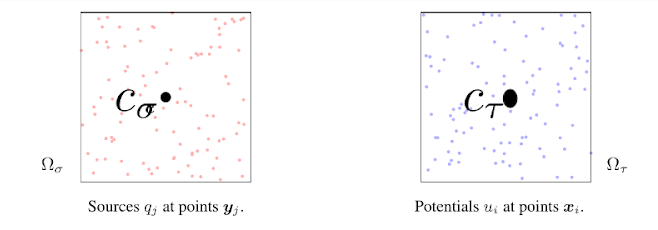
\includegraphics[width=0.8\textwidth]{stboxes}
	\caption{The problem of computing the electrostatic potential between well-separated source and target boxes.}
	\label{fig:stboxes}
\end{figure}

For simplicity, let us switch to complex notation, where each point $\bol x, \bol y \in \R^2$ is reinterpreted as a point in the complex plane $\C$, and with abuse of notation we will write the complex kernel $G(\bol x, \bol y) = \log(\bol x-\bol y)$, where $\log$ is the principal branch of the complex logarithm. The real kernel in \cref{eq:rkernel} is retrieved by taking $\real\{G(\bol x, \bol y)\}$.

We can now formally expand the potential $u_i$ in a Taylor expansion,
\begin{equation}
\begin{aligned}
		u_i &= \sum_{j=1}^{N} \log(\bol x_i-\bol y_j)q_j\\
	&= \sum_{j=1}^{N} \log((\bol x_i-\bol c_\sigma)-(\bol y_j-\bol c_\sigma))q_j\\
	&= \sum_{j=1}^{N} \left[\log(\bol x_i-\bol c_\sigma) + \log\left(1-\frac{\bol y_j-\bol c_\sigma}{\bol x_i-\bol c_\sigma}\right)\right]q_j\\
	&= \sum_{j=1}^{N} \left[\log(\bol x_i-\bol c_\sigma) -\sum_{p=1}^\infty \frac{1}{p} \frac{(\bol y_j-\bol c_\sigma)^p}{(\bol x_i-\bol c_\sigma)^p}\right]q_j\\
	&\approx \log(\bol x_i-\bol c_\sigma)\hat{q}_0^\sigma +\sum_{p=1}^P \frac{1}{p} \frac{1}{(\bol x_i-\bol c_\sigma)^p}\hat{q}_p^\sigma,
\end{aligned}\label{eq:taylor_s}
\end{equation}
where we used the fact that $\log(1-z) = -\sum_p z^p/p$ for $\abs{z}< 1$, the distance $d$ is chosen such that $\abs{\tfrac{\bol y_j-\bol c_\sigma}{\bol x_i-\bol c_\sigma}} < 1$ for every pair of target/source points, and we have approximated the infinite sum by $P$ terms, where $P$ is known as the \textit{interaction rank}. The quantities $\bol{\hat{q}}^\sigma := \{{\hat{q}}_p^\sigma\}_{p=0}^{P-1}$ given by
\begin{equation}
	\begin{aligned}
	\hat{q}_0^\sigma &:= \sum_{j=1}^N q_j,\\
	\hat{q}_p^\sigma &:= \sum_{j=1}^N \frac{-1}{p}(\bol y_j-\bol c_\sigma)^p q_j, \quad p=1,2,\dots,P-1,
	\end{aligned}\label{eq:qhat}
\end{equation}
are the \textit{outgoing expansions} of the source box $\sigma$. On the other hand, the potential $u(x)$ is analytic, thus it can be expanded as a (truncated) Taylor series around the target box center $\bol c_\tau$, 
\begin{align}
u(\bol x_i) = u_i \approx \sum_{p=0}^{P-1}(\bol x_i-\bol c_\tau)^p\bol{\hat{v}}_p^\tau,\label{eq:Ttfi}
\end{align}
where $\bol{\hat{v}}^\tau := \{{\hat{v}}_p^\tau\}_{p=0}^{P-1}$ are the \textit{incoming expansions} of the target box $\tau$. By expanding \cref{eq:taylor_s} in Taylor, and again choosing the distance $d$ large enough, it can be deduced that 
\begin{equation}
	\begin{aligned}
		\hat{v}_0^\tau &= \log(\bol c_\tau-\bol c_\sigma)\hat{q}_0^\sigma + \sum_{p=1}^{P-1}(-1)^p\frac{1}{(\bol c_\sigma-\bol c_\tau)^p} \hat{q}_p^\sigma,\\
		\hat{v}_r^\tau &= -\frac{1}{r(\bol c_\sigma-\bol c_\tau)^r}\hat{q}_0^\sigma + \sum_{p=1}^{P-1}(-1)^p\binom{r+p-1}{p-1}\frac{1}{(\bol c_\sigma-\bol c_\tau)^{r+p}} \hat{q}_p^\sigma, \quad r=1,2,\dots,P-1.
	\end{aligned}\label{eq:vhat}
\end{equation}
Denote $N_\tau$ and $N_\sigma$ the numbers of target and source points, respectively, $\bol q^\sigma := \{q_j\}_{j=1}^{N_\sigma}$ and $\bol u^\tau := \{u_i\}_{i=1}^{N_\tau}$. Note that we have implicitly defined the linear maps
\begin{align}
	\bol{\hat{q}}^\sigma &= \Tbf_\sigma^\text{ofs}\bol q^\sigma, \\
	\bol{\hat{v}}^\tau &= \bol \Tbf_{\tau,\sigma}^\text{ifo} \bol{\hat{q}}^\sigma \quad\text{and}\\
	\bol{u}^\tau &= \bol \Tbf_{\tau}^\text{tfi} \bol{\hat{v}}^\tau,
\end{align}
where $\Tbf_\sigma^\text{ofs}$ is the $P\times N_\sigma$ \textit{outgoing-from-sources} translation operator defined by \cref{eq:qhat}, $\Tbf_\sigma^\text{ifo}$ is the $P\times P$ \textit{incoming-from-outgoing} translation operator defined by \cref{eq:vhat} and $\Tbf_\sigma^\text{tfi}$ is the $N_\tau\times P$ \textit{target-from-incoming} translation operator defined by \cref{eq:Ttfi}. With this, we have effectively computed a \textit{rank-$P$} approximation of the potential
\begin{align}
	\bol{u}^\tau \approx \Tbf_{\tau}^\text{tfi}\left(\Tbf_{\tau,\sigma}^\text{ifo}\left(\Tbf_\sigma^\text{ofs}\bol q^\sigma\right)\right), \label{eq:uhat_approx}
\end{align}
which takes $\bigo{P(N_\sigma+N_\tau) + P^2}$ operations, much less than the $\bigo{N_\sigma N_\tau}$ operations of the naive method for \cref{eq:dir_pot}.\\
Let us introduce the concept of \textit{well separated} boxes, which gives us an estimate of the error committed in \cref{eq:uhat_approx}. We will say that a box $\Omega_\tau$ of center $\bol{c}_\tau$ is \textit{well separated} from a box $\Omega_\sigma$ of center $\bol{c}_\sigma$ and side length $2a$ if 
\begin{align}
	\norm{\bol{c}_\tau-\bol{c}_\tau} \geq 4a.
\end{align}
Now, for \textit{well separated} source and target boxes of the same size, $\Omega_\sigma$ and $\Omega_\tau$, the error committed in \cref{eq:uhat_approx} using a \textit{rank-$P$} approximate potential $\bol u_P^\tau$ is given by
\begin{align}
	\norm{\bol u^\tau-\bol u_P^\tau}_\infty \leq \frac{\eta^P}{P(1-\eta)}\norm{\bol q^\sigma}_1,
\end{align}
where $\eta = \sqrt{2}/(4-\sqrt{2}) \approx 0.547$. This bound can be derived by considering the remainders of the Taylor expansions of \cref{eq:Ttfi} and \cref{eq:taylor_s}, and the definition of \textit{well separated} boxes. It follows that the error decays exponentially with respect to the interaction rank $P$, and we can pick $P=\Ocal(\log(1/\epsilon))$ to achieve an error of $\epsilon$.

\section{The Fast Multipole Method for an uniform cluster of charges}

Consider an uniform cluster of $N$ points $\bol x_i$ with associated charges $q_i$, $i=1,\dots,N$, as shown in \cref{fig:unif_points}. We wish to compute the electrostatic potential at every point $\bol x_i$, this is

\begin{align}
	u(\bol x_i) := u_i = \sum_{j=1}^{N} G(\bol x_i, \bol x_j)q_j, \quad i = 1,2,\dots,N. \label{eq:pot_unif}
\end{align}

\begin{figure}[h!]
	\centering
	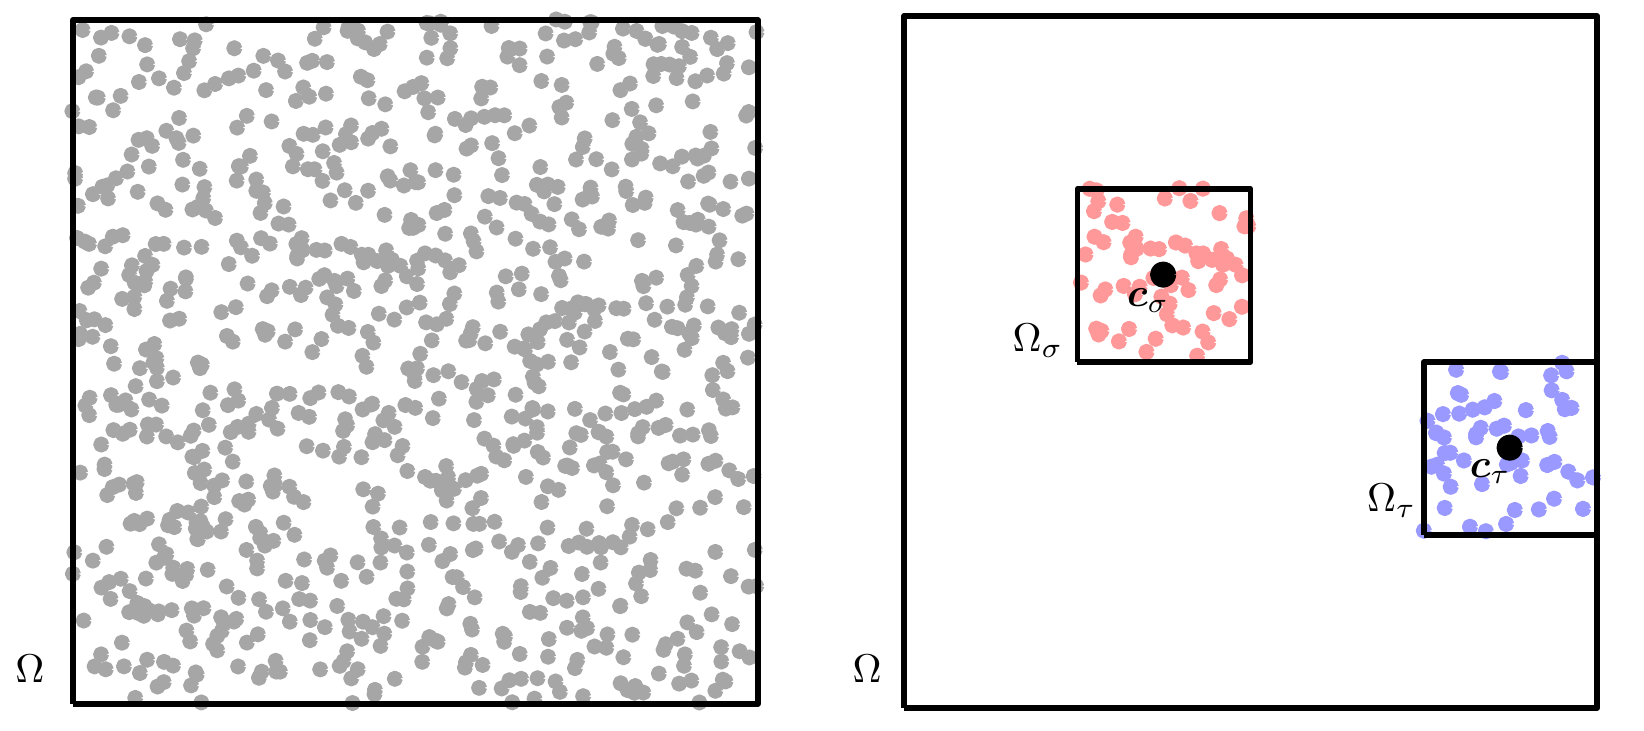
\includegraphics[width=0.8\textwidth]{unif_points}
	\caption{Left: uniform cluster of charges. Right: for \textit{well separated} boxes inside the domain, we could resort to the fast multipole approach of \cref{sec:multipole}.}
\label{fig:unif_points}
\end{figure}

As before, computing the potentials using the naive formula \cref{eq:pot_unif} takes $\Ocal(N^2)$ operations. Here, we will describe the Fast Multipole Method (FMM), which allows us to compute all potentials with only $\Ocal(N)$, using the multipole technique presented in \cref{sec:multipole}.\\
In the FMM we construct a \textit{quadtree} of boxes, a hierarchical tree data structure, where we start with a \textit{root} box which is divided into four smaller and identical \textit{children} boxes. The children constitute the first level of the tree. To construct the second level, each child is again subdivided into four smaller and identical children. This process gets repeated until we reach a prescribed number of levels $L+1$, where level 0 corresponds only to the root box, whereas level $L$ contains the finer boxes, the \textit{leaves}. An example of a quadtree structure with $L=3$ is shown in \cref{fig:tree}.

\begin{figure}[h!]
	\centering
	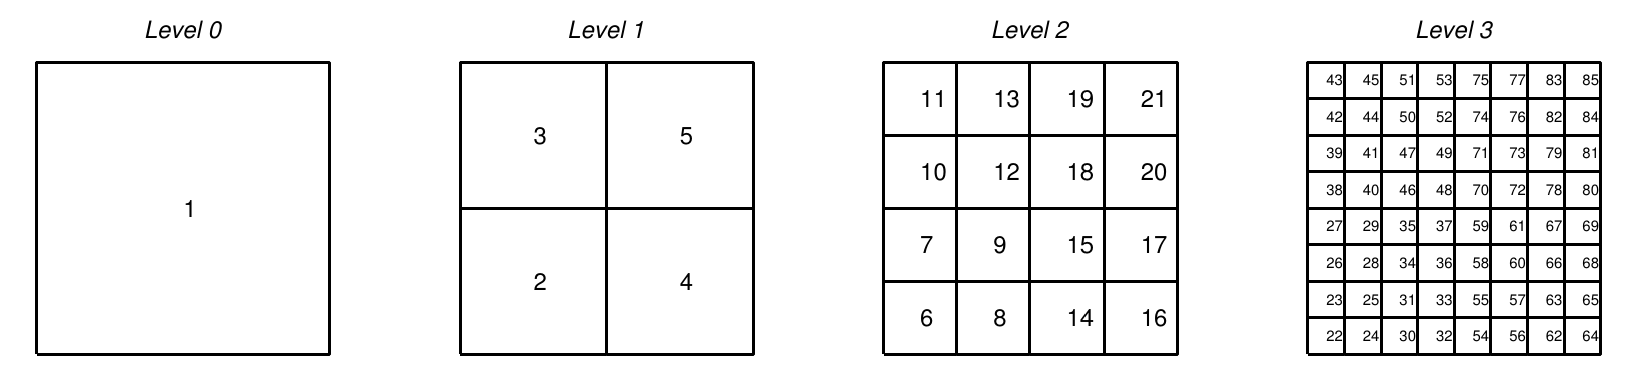
\includegraphics[width=0.8\textwidth]{tree}
	\caption{Quadtree of boxes with $L+1$ levels, $L=3$.}
	\label{fig:tree}
\end{figure}

The idea of this hierarchical data structure is the following. Leaf boxes compute the potentials at their points using multipole expansions for \textit{well separated} boxes and direct evaluations for neighboring boxes and self-interactions. For \textit{closer} well separated boxes we use the multipole expansion shown in \cref{sec:multipole}. This set of \textit{closer} well separated boxes is known as the \textit{interaction list} $\mathcal{L}_\sigma^\text{int}$ of the leaf box $\sigma$, we will provide a precise definition below. Instead, for farther away boxes, it is much more efficient that the leaves' parents compute the multipole interactions (\textit{outgoing} or \textit{incoming} expansions) for the parent's \textit{interaction list}, and then they pass the interaction to their children. Again, if two \textit{well separated} parent boxes are very far away (meaning that they do not belong to each others \textit{interaction list}) then it is more efficient that the parents' parents compute the interaction and so on. This hierarchical transfer of information is the secret behind FMM which allows to achieve a $\Ocal(N)$ complexity. In the end, boxes only care about boxes in their interaction list. If they are farther away, then their ancestry (parents, grandparents, etc.) compute the interaction. And for leaf boxes, they have to care about their interaction list, neighbors and self interactions to finally compute the potentials at their points.

Before describing the FMM algorithm, we will explain how children/parents boxes transfer their \textit{outgoing/incoming expansions} to each other. First, a parent box $\tau$ needs to compute its \textit{outgoing expansion} $\bol{\hat{q}}^\tau$. In fact, this can be done exactly (without any approximation) using the \textit{outgoing expansions} of their children, as shown next. Fix a child box $\sigma$ of $\tau$. Denote $I_\sigma=\{i:\; \bol x_i\in \Omega_\sigma\}$. Its outgoing expansion of order $p$ is
\begin{align}
	\hat{q}_p^\sigma &= \sum_{j\in I_\sigma} \frac{-1}{p}(\bol x_j-\bol c_\sigma)^p q_j,
\end{align}
where $p=1,2,\dots,P-1$. On the other hand, we can write the order $k=1,2,\dots,P-1$ \textit{outgoing expansion} of $\tau$ given by the charges at $\Omega_\sigma$ as
\begin{align}
	\hat{q}_k^{\tau,\sigma} &= \sum_{j\in I_\sigma} \frac{-1}{k}(\bol y_j-\bol c_\tau)^k q_j\\
	&=\sum_{j\in I_\sigma} \frac{-1}{k}((\bol y_j-\bol c_\sigma) - (\bol c_\sigma-\bol c_\tau))^k q_j\\
	&= \sum_{j\in I_\sigma} \frac{-1}{k}\sum_{p=0}^{k} \binom{k}{p} (\bol c_\sigma-\bol c_\tau)^{k-p}(\bol y_j-\bol c_\sigma)^p q_j	\\
	&= \frac{-1}{k} (\bol c_\sigma-\bol c_\tau)^{k}\hat{q}_0^\sigma + \sum_{p=1}^{k} \frac{-1}{k}\binom{k}{p} (\bol c_\sigma-\bol c_\tau)^{k-p}\sum_{j\in I_\sigma}(\bol y_j-\bol c_\sigma)^p\\
	&= \frac{-1}{k} (\bol c_\sigma-\bol c_\tau)^{k}\hat{q}_0^\sigma + \sum_{p=1}^{k} \frac{p}{k}\binom{k}{p} (\bol c_\sigma-\bol c_\tau)^{k-p}\sum_{j\in I_\sigma}\frac{-1}{p}(\bol y_j-\bol c_\sigma)^p\\
	&= \frac{-1}{k} (\bol c_\sigma-\bol c_\tau)^{k}\hat{q}_0^\sigma + \sum_{p=1}^{k} \frac{p}{k}\binom{k}{p} (\bol c_\sigma-\bol c_\tau)^{k-p}\hat{q}_p^\sigma. \label{eq:Tofo}
\end{align}

This defines a linear operator $\Tbf_{\tau,\sigma}^\text{ofo}$, known as the $P\times P$ \textit{outgoing-from-outgoing} translation operator, which maps the \textit{outgoing expansion} $\bol{\hat{q}}^{\sigma}$ of the child $\sigma$ into the parent $\tau$ expansion $\bol{\hat{q}}^{\tau}$. This definition of $\Tbf_{\tau,\sigma}^\text{ofo}$ is slightly different to the one shown in \cite{martinsson2019fast}. Finally, the \textit{total outgoing expansion} of $\tau$ is given by the sum of the contributions of their children, this is
\begin{align}
	\bol{\hat{q}}^{\tau} = \sum_{\sigma \in \Lcal_\tau^\text{child}} \Tbf_{\tau,\sigma}^\text{ofo} \bol{\hat{q}}^{\sigma},
\end{align}
where $\Lcal_\tau^\text{child}$ is the set of children of $\tau$.

Once a parent $\tau$ computes its \textit{incoming expansion} $\bol{\hat{v}}^{\tau}$ using the \textit{outgoing expansions} of the boxes in its interaction list, it needs to transfer this \textit{incoming expansion} to each of its four children. Fix a children $\sigma$ of $\tau$. Its \textit{incoming expansion} is given by
\begin{align}
	\bol{\hat{v}}^{\sigma} = \Tbf_{\tau,\sigma}^\text{ifi}\bol{\hat{v}}^{\tau} + \sum_{\nu\in\Lcal_\sigma^\text{int}} \Tbf_{\sigma,\nu}^\text{ifo}\bol{\hat{q}}^{\nu},
\end{align}
where the first term is the contribution from the parent (this includes the contribution of boxes farther away than the interaction list $\Lcal_\sigma^\text{int}$ of $\sigma$), and the second term correspond to the contribution of the interaction list $\Lcal_\sigma^\text{int}$ of $\sigma$. The linear operator $\Tbf_{\sigma,\tau}^\text{ifi}$ is the $P\times P$ \textit{incoming-from-incoming} translation operator, which maps the \textit{incoming expansion} $\bol{\hat{v}}^{\tau}$ of the parent $\tau$ into the child $\sigma$ expansion $\bol{\hat{v}}^{\sigma}$. Using the expression \cref{eq:Ttfi} and the same binomial expansion tricks as used in \cref{eq:Tofo}, it can be derived that
\begin{align}
	\Tbf_{\sigma,\tau}^\text{ifi} = \begin{cases}
		\binom{p}{r}(\bol c_\sigma-\bol c_\tau)^{p-r},\quad&\text{for }r\leq p,\\
		0, &\text{for }r> p,
	\end{cases}
\end{align}
for $p,r=0,1,\dots,P-1$.

For a box $\tau$ let us define the following:
\begin{itemize}
	\item The parent of $\tau$ is the box on the next coarsest level that contains $\tau$.
	\item The children list of $\tau$ is the set $\Lcal_\tau^\text{child}$ of boxes whose parent is $\tau$.
	\item The neighbor list of $\tau$ is the set $\Lcal_\tau^\text{nei}$ of boxes on the same level that directly touch $\tau$.
	\item The interaction list of $\tau$ is the set $\Lcal_\tau^\text{int}$ of all boxes $\sigma$ such that (1) $\sigma$ and $\tau$ are on the same level, (2) $\sigma$ and $\tau$ do not touch, and (3) the parents of $\sigma$ and $\tau$ do touch.
	\item Denote $A(I_\tau,I_\sigma)$ as the (dense) operator that maps the charges $\bol q^\sigma$ at box $\sigma$ into the potentials $\bol u^\tau$ at box $\tau$, i.e., $\bol u^\tau=A(I_\tau,I_\sigma)\bol q^\sigma$.
\end{itemize}

\begin{figure}[h!]
	\centering
	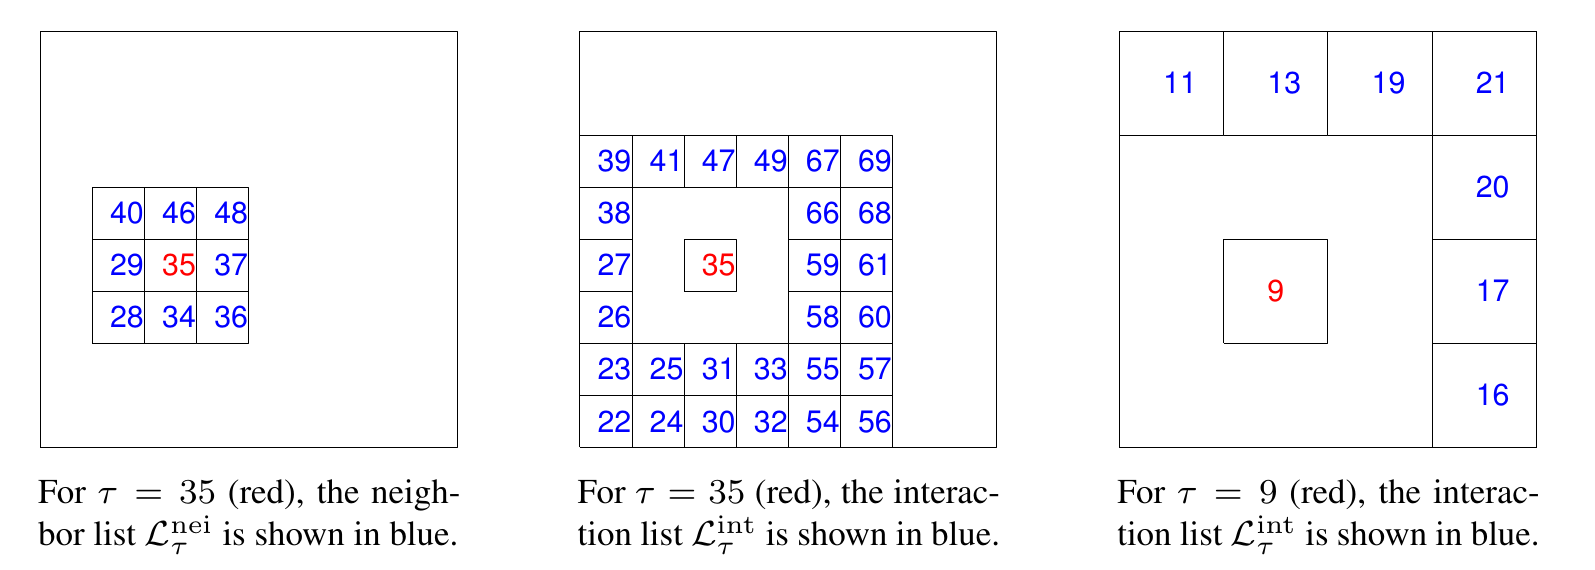
\includegraphics[width=0.8\textwidth]{ilist}
	\caption{Examples of interaction and neighbor lists.}
	\label{fig:ilist}
\end{figure}

A diagram that shows an example of interaction and neighbor lists is presented in \cref{fig:ilist}. Now we have all the tools to describe the FMM algorithm. In the precomputation step we first assemble the quadtree, the boxes lists and precompute all of the translation operators. Now, to compute the potentials $\bol u$ for a given set of charges $\bol q$ we follow three steps:
\begin{enumerate}
	\item Upward pass: compute the \textit{outgoing expansions} of all boxes. Start at the finest level computing the expansions directly from the charges. For parent boxes, compute their expansions using their children's expansions.
	\item Downward pass: compute the \textit{incoming expansions} of all boxes. From level $l=2$ to the finest, compute the \textit{incoming expansions} using the parent's contribution and the interaction list's contribution.
	\item Compute potentials: Each leaf computes the potentials at its points, using the incoming expansions and direct evaluations of the potentials for neighboring boxes and self-interactions.
\end{enumerate}
The FMM algorithm is detailed in \cref{fig:upfmm}, \cref{fig:downfmm} and \cref{fig:potfmm}.
\begin{figure}[h!]
	\centering
	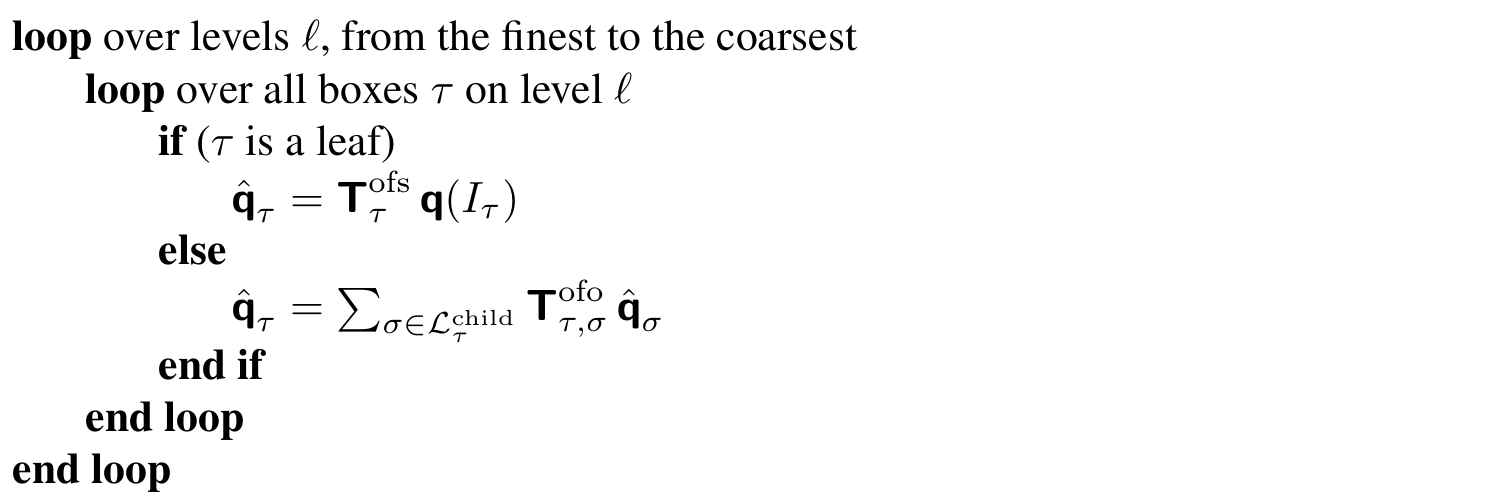
\includegraphics[width=0.8\textwidth]{upfmm}
	\caption{FMM upward pass.}
	\label{fig:upfmm}
\end{figure}
\begin{figure}[h!]
	\centering
	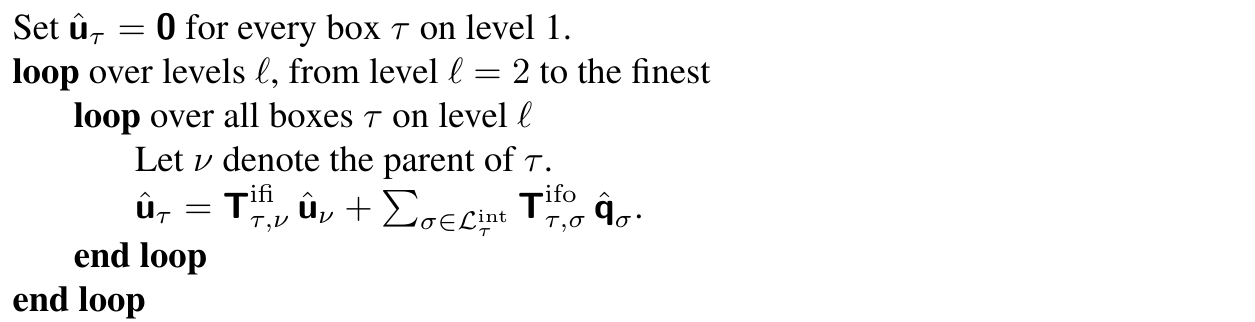
\includegraphics[width=0.8\textwidth]{downfmm}
	\caption{FMM downward pass.}
	\label{fig:downfmm}
\end{figure}
\begin{figure}[h!]
	\centering
	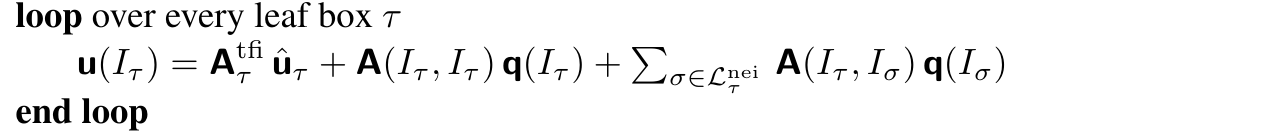
\includegraphics[width=0.8\textwidth]{potfmm}
	\caption{FMM compute potentials step.}
	\label{fig:potfmm}
\end{figure}

\section{Error estimation}
The error for FMM type of methods is usually estimated using a single translation operation, which includes the processes that maps charges into \textit{outgoing expansions}, into \textit{incoming expansions} and finally into potentials. As shown in \cref{sec:multipole}, this error $\epsilon$ decays exponentially fast with respect to the interaction rank  


\bibliographystyle{siamplain}
\bibliography{references}

\end{document}
